\providecommand{\main}{../..}

\documentclass[../../thesis]{subfiles}


\begin{document}

\chapter{Kiến thức nền tảng}

Chương này giới thiệu sơ qua về các nền tảng trong quá trình xây dựng ứng dụng.

\begin{itemize}
    \item
        Hai nền tảng đầu tiên liên quan đến nhau, là tiền đề cho toàn bộ ứng
        dụng sẽ được giới thiệu trước, gồm hệ điều hành Android và ngôn ngữ lập
        trình Kotlin.
    \item
        Tiếp theo, lựa chọn về kiến trúc tổng quan, liên quan đến giao diện của
        ứng dụng được trình bày.
    \item
        Sau đó, cơ sở dữ liệu một số phần mở rộng của nó dùng trong ứng dụng sẽ
        được nhắc qua.
    \item
        Cuối cùng là thông tin về \texttt{.cbz} - định dạng tệp tin mà ứng dụng
        đọc, gồm hai phần: sơ lược về định dạng \texttt{.zip} mà \texttt{.cbz}
        dựa trên, và các trường metadata trong tệp tin \texttt{.cbz} - nguồn
        thông tin quan trọng để quản lí truyện.
\end{itemize}


%----------------------------------------------------------------------------------------
%	2.1: Hệ điều hành Android
%----------------------------------------------------------------------------------------

\section{Hệ điều hành Android}

Android là một hệ điều hành do Google phát triển cho thiết bị di động. Android
dùng nhân Linux và được thiết kế cho màn hình cảm ứng. Cùng với iOS của Apple,
Android trở thành một phần không thể thiếu của cuộc cách mạng di động bắt đầu
vào cuối những năm 2000.

Google mua lại phiên bản Android đầu của công ty khởi nghiệp cùng tên vào năm
2005, và phát triển hệ điều hành này từ đó. Ngoài Google, Android còn nhận đóng
góp lớn từ cộng đồng, do là một dự án mã nguồn mở (phần lớn mã nguồn dùng giấy
phép Apache); tên chính thức của dự án là Android Open Source Project. Dù vậy,
mọi thiết bị Android thương mại đều có ứng dụng độc quyền. Ví dụ đáng kể là bộ
Google Mobile Service, chứa những ứng dụng không thể thiếu như trình duyệt
Chrome hay chợ Play Store. Về mặt này, Android khá giống Chrome: thành phần cốt
lõi kĩ thuật được phát triển theo mô hình mã nguồn mở (AOSP và Chromium), còn
thành phần liên quan đến trải nghiệm người dùng được phát triển riêng.

\begin{wrapfigure}{r}{8.6cm}
    \centering
    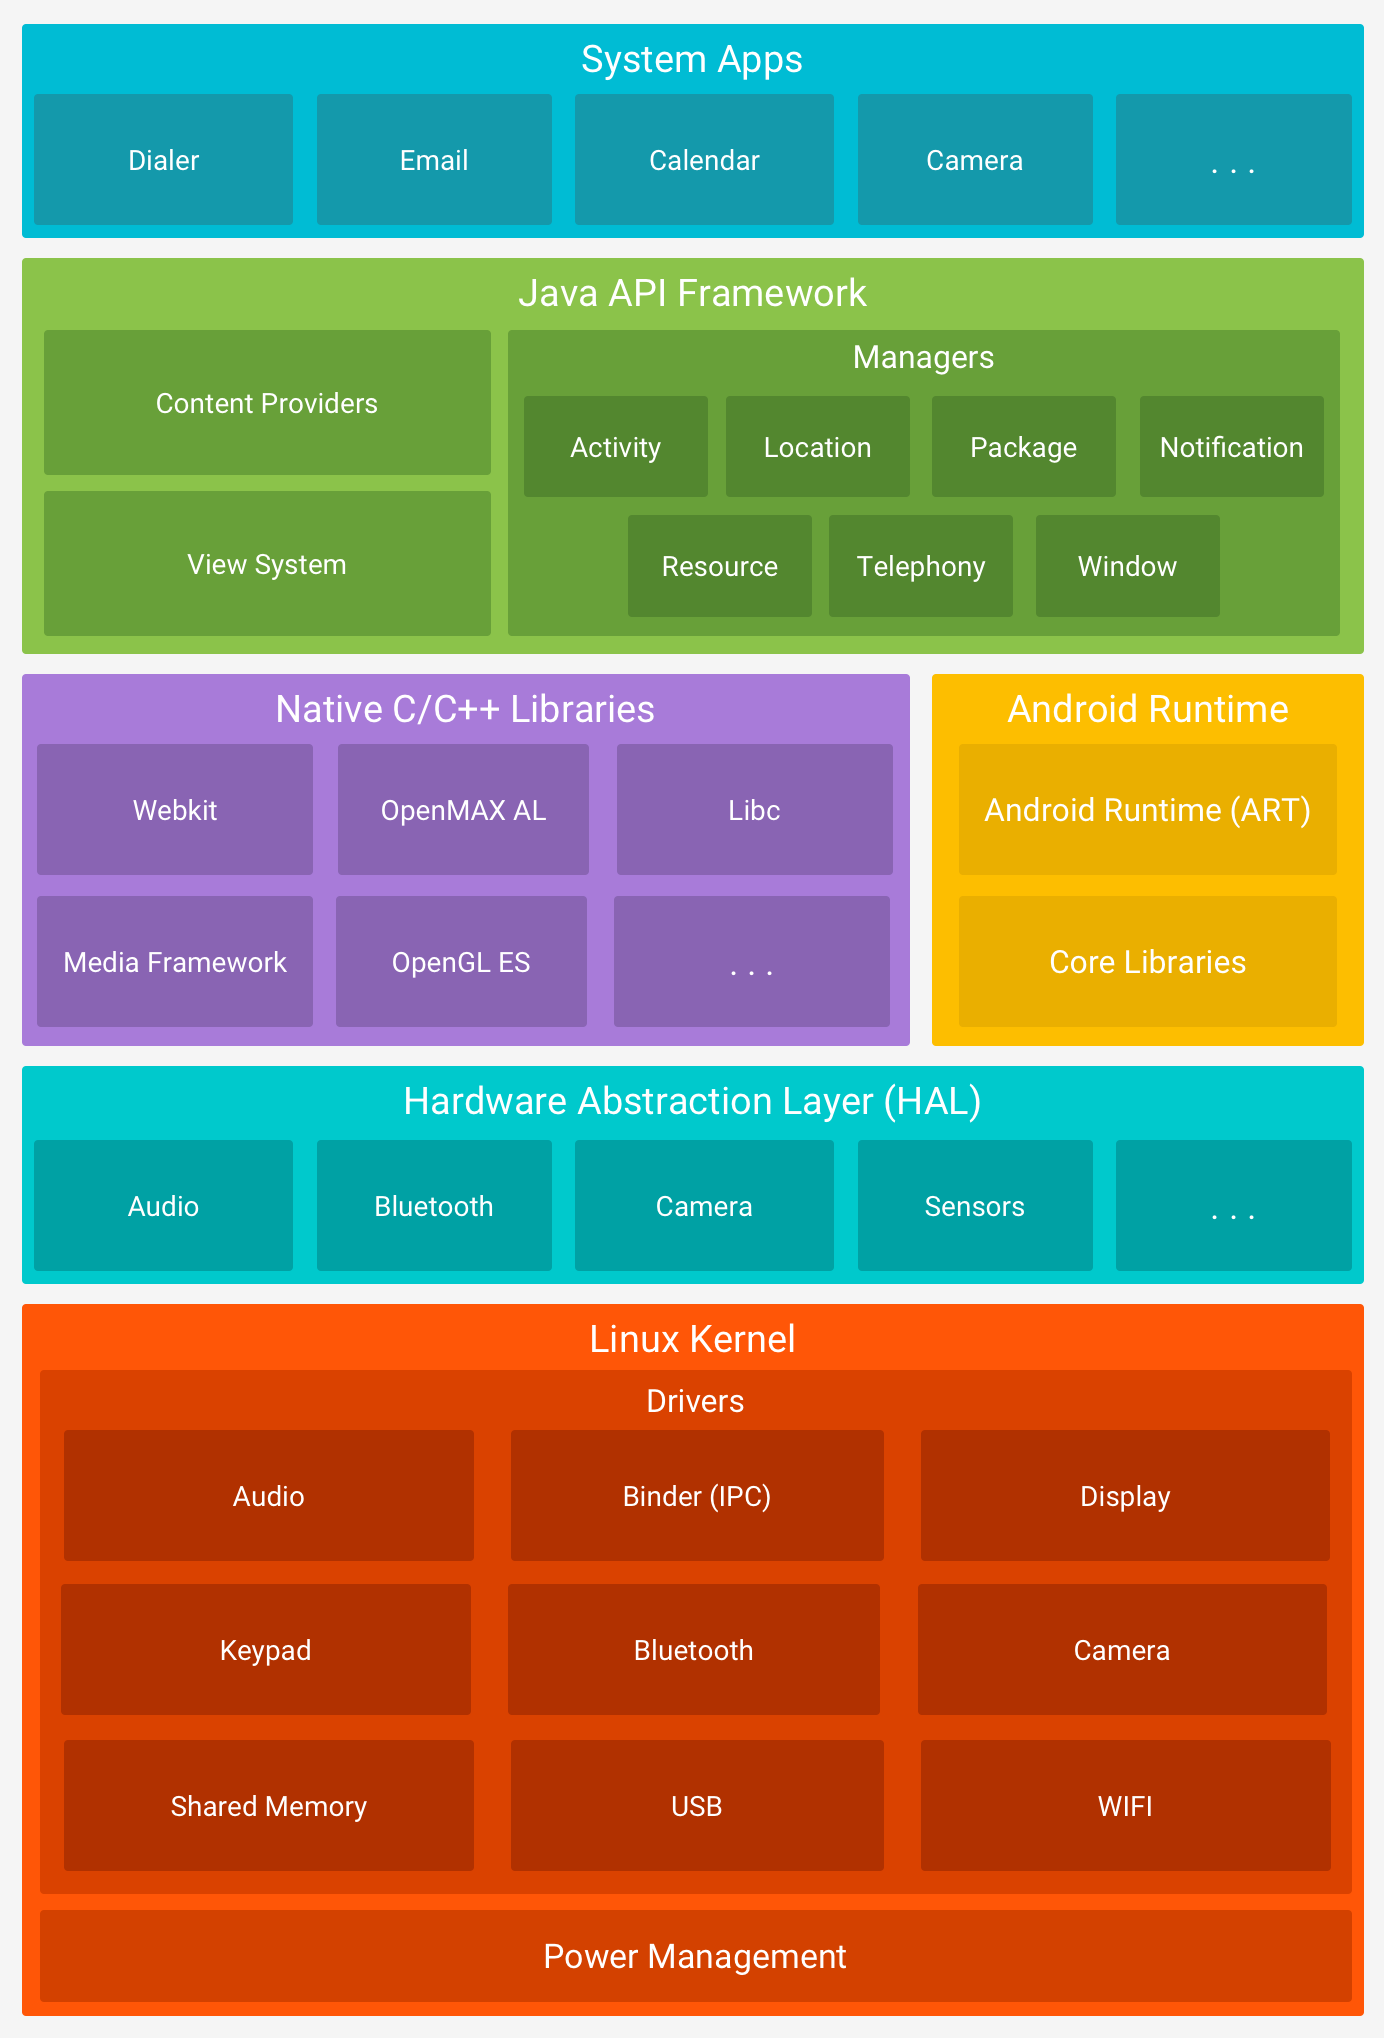
\includegraphics[width=\linewidth]{../images/android-stack_2x.png}
    \vspace*{-10mm}
    \caption{Các phân lớp của Android}
    \label{fig:android-stack}
\end{wrapfigure}

Hệ điều hành Android được phân lớp như sau:

\begin{itemize}
    \item
        Nhân Linux (Linux Kernel):

        Đây là tầng thấp nhất. Android dùng nhánh hỗ trợ dài hạn (LTS) của
        Linux. Không như kiểu phát triển distro trên máy tính (chủ yếu thay đổi
        ở ngoài nhân), Google sửa và thêm bớt nhiều thành phần vào nhân trước
        khi tích hợp.
    \item
        Lớp phần cứng trừu tượng (Hardware Abstraction Layer):

        Tầng này trừu tượng hóa các chi tiết phần cứng bằng cách đưa ra các giao
        diện chung cho một kiểu phần cứng nào đó, giúp các tầng trên không cần
        quan tâm đến chi tiết riêng của phần cứng.

    \item
        Android Runtime (ART):

        Ứng dụng Java cần thêm một ứng dụng để chuyển bytecode thành mã máy.
        Trên desktop, đó là các máy ảo Java (JVM). Trên Android, Android Runtime
        nhận nhiệm vụ này. Hai máy ảo này khác nhau ở chỗ ART \emph{biên dịch}
        bytecode thành mã máy (trước khi chạy - AOT), còn JVM \emph{thông dịch}
        bytecode thành mã máy (trong khi chạy).

        ART hiện hỗ trợ đa số tính năng của Java 8.
\end{itemize}

% Split itemize to avoid confusing wrapfigure
% https://tex.stackexchange.com/a/285760/206774
\begin{itemize}[resume, before = \vspace*{-\dimexpr\topsep+\partopsep\relax}]
    \item
        Thư viện C/C++:

        Tầng thư viện native nằm ngang hàng với ART, phục vụ các tiến trình hệ
        thống và một số ứng dụng dùng NDK (tức gọi API C cấp thấp) như trò chơi
        điện tử.
    \item
        Khung phát triển ứng dụng (Java API Framework):

        Mọi ứng dụng Java được viết nhờ sử dụng các thành phần của tầng này
        thông qua API Java. Tầng này cung cấp toàn bộ tính năng của Android cho
        lập trình viên, bao gồm các yếu tố cơ bản như giao diện (View System),
        truy xuất,\ldots{}

        Lập trình viên có quyền truy cập vào lớp này tương đương với ứng dụng hệ
        thống. Đây có thể coi là một cam kết tránh độc quyền công nghệ, tức đa
        số ứng dụng hệ thống không có khả năng đặc biệt, hay hiệu năng cao hơn
        ứng dụng bên thứ ba tương tự.
    \item
        Ứng dụng hệ thống (System Apps)

        Android đi kèm với một số ứng dụng hệ thống như ứng dụng SMS, trình
        duyệt, lịch,\ldots{} Google cho phép thay thế đa số các ứng dụng này với
        ứng dụng bên thứ ba, tuy nhiên có những ngoại lệ như ứng dụng Cài đặt
        (Settings).
\end{itemize}

Gần như mọi ứng dụng Android cơ bản đều sử dụng thành phần View System trong
tầng Khung phát triển để viết giao diện, và yacv không là ngoại lệ. yacv còn sử
dụng thành phần Content Provider, cụ thể là bộ Storage Access Framework, và sẽ
được đề cập ở các phần sau.

\subsection{Android Jetpack}

Jetpack là bộ thư viện giúp viết ứng dụng Android nhanh gọn, ít lỗi hơn so với
việc tự viết những đoạn mã tương tự. Jetpack gồm hai thành phần:

\begin{itemize}
    \item
        AndroidX: đưa \emph{API} của phiên bản hệ điều hành mới lên máy cũ
    \item
        Architecture Component: đưa ra \emph{thư viện} hoàn toàn mới
\end{itemize}

Việc cập nhật Android rất khó khăn do phải chờ nhà sản xuất tối ưu. Do đó,
Google viết AndroidX, trước gọi là Thư viện Hỗ trợ (Support Library), để đưa API
Android mới lên máy cũ. Chú ý rằng Jetpack chỉ có ích cho lập trình viên (API
mới tiện hơn thực ra là wrapper của API sẵn có), chứ không cập nhật tính năng hệ
điều hành.

yacv sử dụng nhiều thành phần của Jetpack, trong đó đáng kể đến ba thư viện sau:

\begin{itemize}
    \item
        LiveData: giúp giao diện luôn được cập nhật theo dữ liệu mới nhất
    \item
        ViewModel: giúp tách dữ liệu và giao diện
    \item
        Room: giúp việc lưu dữ liệu trong SQLite thuận tiện hơn
\end{itemize}

Room là một phần quan trọng của yacv, do đó sẽ được giới thiệu chi tiết ở
\protect\hyperlink{P2.4.2-room}{mục sau}.


%----------------------------------------------------------------------------------------
%	2.2: Ngôn ngữ lập trình Kotlin
%----------------------------------------------------------------------------------------

\section{Ngôn ngữ lập trình Kotlin}

Java là ngôn ngữ lập trình đầu tiên được hỗ trợ trên Android, nhưng không phải
duy nhất. Từ 2019, Google khuyên lập trình viên viết ứng dụng trên Kotlin, một
ngôn ngữ mới do JetBrains phát triển. Giới thiệu lần đầu vào năm 2011, Kotlin
được định hướng trở thành lựa chọn thay thế cho Java. Điều đó thể hiện ở việc
Kotlin tương thích hoàn toàn với Java (từ Java gọi được Kotlin và ngược lại), do
cùng được biên dịch thành JVM bytecode.

Điểm mạnh của Kotlin so với Java là tính ngắn gọn. Do được phát triển mới,
Kotlin không cần tương thích với phiên bản cũ, cho phép dùng các cú pháp hiện
đại, gọn ghẽ. Ngoài ra, vì được một công ty tư nhân phát triển, Kotlin không cần
chờ đến các cuộc họp phức tạp để đạt đồng thuận về tính năng mới, giúp ngôn ngữ
liên tục được cải tiến. Đồng thời, công ty cũng mở mã nguồn của Kotlin và chương
trình dịch, giúp đẩy nhanh quá trình phát triển và tạo thiện cảm cộng đồng cho
một ngôn ngữ non trẻ.

Sau đây là tóm tắt một số đặc điểm kĩ thuật của Kotlin:

\begin{itemize}
    \item
        Về mô hình, Kotlin hỗ trợ hướng đối tượng như Java, nhưng còn có hướng
        hàm, thể hiện ở tính năng hàm ẩn danh (lambda), và hàm được coi là
        first-class.
    \item
        Về hệ thống kiểu, Kotlin giống hệt Java:

        \begin{itemize}
            \item
                Là kiểu tĩnh (statically typed), tức kiểu được kiểm tra khi biên
                dịch (thay vì khi chạy, như Python, JavaScript,\ldots)
            \item
                Là kiểu mạnh (strongly typed), tức không cho phép chuyển kiểu
                ngầm
        \end{itemize}
    \item
        Về cú pháp, Kotlin gọn và hiện đại: bỏ dấu \texttt{;} cuối dòng,
        template literal,\ldots{}
    \item
        Về lỗi, Kotlin luôn được quảng cáo về khả năng chống
        \texttt{NullPointerException}. Kotlin ``né'' lỗi này do buộc người viết
        đánh dấu cụ thể rằng một đối tượng có thể bị \texttt{null} hay không
        bằng hậu tố \texttt{?} ở khai báo kiểu. Từ đó, Kotlin biết chính xác đối
        tượng có thể là \texttt{null} hay không, và buộc xử lí nếu có.
\end{itemize}

Do Google khuyên dùng Kotlin khi viết ứng dụng Android, tôi cho rằng khóa luận
này là một cơ hội phù hợp để thử Kotlin thay vì dùng Java quen thuộc, và quyết
định chọn viết yacv bằng Kotlin.

\subsection{Coroutine}

\subsubsection{Giới thiệu}

Một thư viện quan trọng của kotlin là \emph{coroutine}. Coroutine giúp viết ứng
dụng có tính tương tranh (concurrency) và bất đồng bộ (asynchronous) một cách
đơn giản hơn.

Về cơ bản, coroutine giống với luồng (thread), nhưng nhẹ hơn. Coroutine luôn
dùng mô hình \emph{đa nhiệm hợp tác} (cooperative multitasking), khác với luồng
hay dùng đa nhiệm ưu tiên (preemptive multitasking). Mấu chốt khác biệt của
chúng là đa nhiệm hợp tác có các ``điểm dừng'' do người viết tạo; khi chạy đến
đó, coroutine có thể dừng lại, chủ động nhả CPU cho việc khác, rồi tiếp tục việc
đang dở vào lúc thích hợp. Ngược lại, đa nhiệm ưu tiên có thể buộc một luồng
đang chạy ngừng lại bất kì lúc nào để ưu tiên chạy một luồng khác. Đây cũng là
điểm khiến coroutine nhẹ hơn: chi phí chuyển ngữ cảnh (context switching) được
kiểm soát và cắt giảm, do chuyển sang thực thi một coroutine khác chưa chắc đã
chuyển sang một luồng hệ điều hành khác.

Với những điều trên, coroutine chưa làm được nhiều. Roman Elizarov, trưởng dự án
Kotlin, hướng coroutine trong Kotlin theo một ý tưởng mới: \emph{tương tranh có
cấu trúc} (structured concurrency, từ đây gọi tắt là SC). Ý tưởng này tiếp tục
đơn giản hóa việc viết những đoạn mã tương tranh bằng cách áp đặt một số giới
hạn, cấu trúc cơ bản. Kết quả là coroutine trong Kotlin hỗ trợ việc xử lí lỗi và
ngừng tác vụ bất đồng bộ tốt hơn việc dùng luồng, hay các thư viện tương tranh
như RxJava.

Coroutine được dùng để tăng tốc những đoạn mã chạy chậm trong yacv (sẽ được mô
tả sau). Ngoài cải thiện về hiệu năng, coroutine và tương tranh có cấu trúc còn
cho phép viết mã ngắn gọn, rõ ràng hơn. Do có tác động lớn, coroutine sẽ được
giới thiệu kĩ hơn ở phần này.

\subsubsection{Bài học từ quá khứ: lập trình có cấu trúc}

\begin{wrapfigure}{r}{5cm}
    \centering
    \vspace*{-6mm}
    \includesvg[width=\linewidth]{../images/sequential-and-go-to-schematic.svg}
    \vspace*{-10mm}    % Manually make figure & caption closer together
    \caption{Lập trình phi cấu trúc với \texttt{GOTO}}
    \label{fig:non-structured-programming}
\end{wrapfigure}

Để hiểu về SC, ta có thể so sánh nó với \emph{lập trình có cấu trúc} (structured
programming). Để hiểu sơ về lập trình có cấu trúc, ta phải tìm về \emph{lập
trình phi cấu trúc} (non-structured programming), với đặc điểm là lệnh nhảy
\texttt{GOTO}. Trong buổi đầu của máy tính, lệnh này được dùng nhiều vì hợp với
cách máy tính chạy.

Vấn đề của lập trình phi cấu trúc, hay của \texttt{GOTO}, có thể tóm gọn như
sau:

\begin{itemize}
    \item
        Khó nắm bắt luồng chương trình

        Khi đã chạy \texttt{GOTO}, các lệnh phía sau nó không biết khi nào mới
        chạy, vì chương trình chuyển sang lệnh khác mà không trở lại. Luồng chạy
        trở thành một đống ``mì trộn'' như Hình 3, thay vì tuần tự từ trên
        xuống. Tệ hơn, tính trừu tượng bị phá vỡ: khi gọi hàm, thay vì có thể bỏ
        qua chi tiết bên trong, ta phải biết rõ để xem có lệnh nhảy bất ngờ nào
        không.
\end{itemize}

% \begin{wrapfigure}{l}{5cm}
%     \centering
%     \includesvg[width=\linewidth,inkscapelatex=false]
%         {../images/flow-matic-4.svg}
%     \caption{Sự lộn xộn của lập trình phi cấu trúc}
%     \label{fig:goto-spaghetti}
% \end{wrapfigure}

\begin{itemize}[resume, before = \vspace*{-\dimexpr\topsep+\partopsep\relax}]
    \item
        Không cài đặt được các chức năng mới (ngoại lệ, quản lí tài nguyên tự
        động,\ldots)

        Xét ví dụ Java sau về quản lí tài nguyên tự động:

        \begin{minted}{Java}
        try (Scanner scanner = new Scanner(new File("f.txt"))) {
            goto(SOMEWHERE);    // Giả sử Java có GOTO
        }
        \end{minted}

        Do không trả lại luồng điều khiển, việc đóng luồng nhập từ tệp cũng
        không chắc chắn xảy ra, dẫn đến rò rỉ tài nguyên, làm khối lệnh vô dụng.

        Điều gần tương tự cũng khiến việc xử lí ngoại lệ và nhiều tính năng khác
        trở nên rất khó đạt được, một khi ngôn ngữ cho phép \texttt{GOTO}.
\end{itemize}

\begin{wrapfigure}{r}{5cm}
    \centering
    \vspace*{-6mm}
    \includesvg[width=\linewidth]{../images/control-schematics.svg}
    \vspace*{-10mm}
    \caption{Ba cấu trúc cơ bản của lập trình có cấu trúc: rẽ nhánh \texttt{if},
        lặp \texttt{for} và gọi hàm}
    \label{fig:3-basic-construct}
\end{wrapfigure}

Lập trình có cấu trúc đơn giản hóa luồng chạy bằng cách giới hạn các lệnh nhảy
còn \texttt{if}, \texttt{for} và gọi hàm. Khác biệt mấu chốt của ba lệnh này so
với \texttt{GOTO} là chúng \emph{trả luồng điều khiển} về điểm gọi, thể hiện rõ
ở \autoref{fig:3-basic-construct}. Theo định nghĩa, ba lệnh trên giải quyết được
hậu quả đầu tiên. Đồng thời, các hậu quả số hai cũng được giải quyết, do ngôn
ngữ đã có cấu trúc (cụ thể là có call stack).

Ngày nay, ba cấu trúc trên đã trở thành phần không thể thiếu trong mọi ngôn ngữ
lập trình, và \texttt{GOTO} chỉ còn dùng trong hợp ngữ. Quá khứ cho thấy nếu áp
dụng một số cấu trúc, giới hạn, ta có thể giải quyết vấn đề một cách tinh tế và
gọn gàng. Trong trường hợp này, SC có thể loại bỏ một số điểm yếu của các API
tương tranh/bất đồng bộ truyền thống, giống cách lập trình có cấu trúc đã làm.

\subsubsection{Áp dụng vào hiện tại: tương tranh có cấu trúc}

Trước hết, ta xem xét hai kiểu API tương tranh hay dùng hiện nay:

\begin{table}[H]
    \begin{tabular}{r r r}
        \toprule
        Tên         & Giải thích                                                 & Ví dụ \\
        \midrule
        Tương tranh & Chạy một hàm theo cách tương tranh với luồng chạy hiện tại & Thread(target=fn).start() \# Python \\
        Bất đồng bộ & Chạy một hàm khi có sự kiện xảy ra (callback)              & element.onclick = cb; // JS \\
        \bottomrule
    \end{tabular}
\end{table}

\begin{wrapfigure}{r}{5cm}
    \centering
    \vspace*{-6mm}
    \includesvg[width=\linewidth]{../images/sequential-and-go-to-schematic.svg}
    \vspace*{-10mm}
    \caption{Tương tranh phi cấu trúc với \texttt{goroutine} - API thuộc kiểu
    tương tranh}
    \label{fig:goroutine}
\end{wrapfigure}

Qua \autoref{fig:goroutine}, không khó để thấy rằng mọi vấn đề của lập trình phi
cấu trúc đều lặp lại với hai API trên:

\begin{itemize}
    \item
        Ta xem lại ví dụ về quản lí tài nguyên tự động. Nếu có luồng thực thi
        khác tương tranh với luồng chính, thì khi luồng chính đóng
        \texttt{Scanner}, có thể luồng kia đang đọc dở. Do đó, tính năng này
        không thể hoạt động.
\end{itemize}

\begin{itemize}[resume, before = \vspace*{-\dimexpr\topsep+\partopsep\relax}]
    \item
        Với tính năng bắt ngoại lệ, nếu có ngoại lệ ở luồng tương tranh, ta cũng
        không có cách nào để biết, và buộc phải kệ nó.
\end{itemize}

Trên thực tế, có cách để thực hiện một số chức năng trên với API hiện tại, tuy
vậy đó đều là cách xử lí riêng, do đó chưa thực sự thuận tiện khi dùng. Ví dụ,
ES6 có \texttt{catch()} để bắt ngoại lệ trong \texttt{Promise} mà không (thể)
dùng cấu trúc \texttt{try-catch} sẵn có. Với SC, các vấn đề này đều được giải
quyết.

Trong \autoref{fig:kotlin-coroutine}, ta xét một đoạn mã tương tranh dùng
coroutine trong Kotlin, tức dùng SC (không phải coroutine trong mọi ngôn ngữ đều
dùng mô hình này).

\begin{wrapfigure}{l}{8cm}
    \centering
    \includesvg[width=\linewidth,inkscapelatex=false]    % To leave text as is
        {../images/kotlin-coroutine.svg}                 % https://tex.stackexchange.com/a/595916/206774
    \vspace*{-10mm}
    \caption{Tương tranh có cấu trúc dùng coroutine trong Kotlin}
    \label{fig:kotlin-coroutine}
\end{wrapfigure}

Nguyên tắc của SC là: \emph{coroutine cha chờ mọi coroutine con chạy xong}, kể
cả khi nó xong trước. Nguyên tắc này đảm bảo rằng khi một hàm kết thúc, không
còn tác vụ tương tranh nữa, và luồng điều khiển hợp nhất được trả về điểm gọi.
Đột nhiên, hai tính năng có vấn đề ở trên lại hoạt động:

\begin{itemize}
    \item
        Quản lí tài nguyên tự động: do đảm bảo trả lại luồng điều khiển, tài
        nguyên đảm bảo được đóng; do không còn tác vụ con, tài nguyên không bị
        đọc sau đóng.
\end{itemize}

\begin{itemize}[resume, before = \vspace*{-\dimexpr\topsep+\partopsep\relax}]
    \item
        Bắt ngoại lệ: do cấu trúc cha-con (khác với các API hiện tại cho rằng
        hai tác vụ tương tranh là ngang hàng), coroutine con có thể ném ngoại lệ
        để coroutine cha bắt.
\end{itemize}

Chú ý là các API hiện tại không phải không làm được nguyên tắc trên, vấn đề là
thực hiện một cách \emph{tự động} và \emph{đảm bảo}. Ví dụ, trong JS, để tuân
theo nguyên tắc này, ta cần \texttt{await} với mọi hàm \texttt{async}; nếu
không, luồng chạy của hàm đó sẽ tách biệt với luồng chương trình, như Hình 5 mô
tả. Do không có ràng buộc chặt chẽ kia, các tính năng ngôn ngữ mới cũng khó cài
đặt như đã phân tích.

Do trong các ngôn ngữ khác, nguyên tắc trên chỉ là một ca sử dụng, việc ép buộc
viết theo ca sử dụng này đòi hỏi lập trình viên thay đổi suy nghĩ về mã tương
tranh. Đổi lại, chương trình trở nên sáng rõ, giống với những đoạn mã viết theo
kiểu tuần tự truyền thống.

Một khi vấn đề tương tranh được giải quyết hoặc đơn giản hóa, việc song song hóa
(paralellization) để tăng tốc ứng dụng chỉ còn là một chi tiết cài đặt.

\end{document}
